% Created by tikzDevice version 0.12.6 on 2024-04-18 18:47:24
% !TEX encoding = UTF-8 Unicode
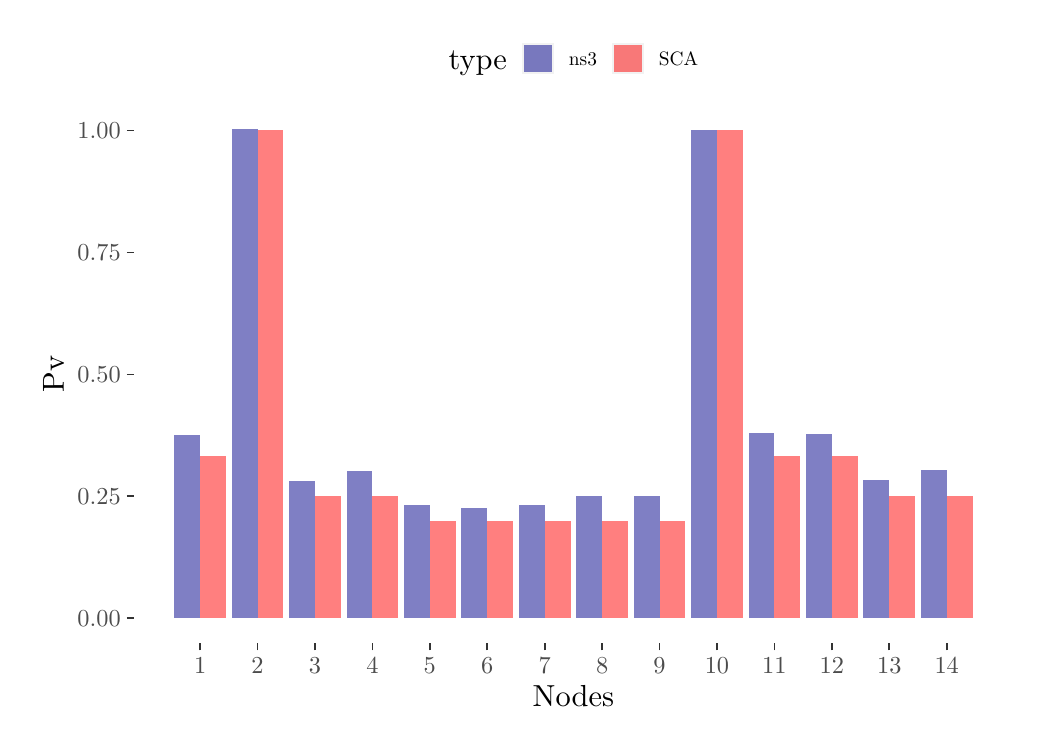
\begin{tikzpicture}[x=1pt,y=1pt]
\definecolor{fillColor}{RGB}{255,255,255}
\path[use as bounding box,fill=fillColor,fill opacity=0.00] (0,0) rectangle (361.35,252.94);
\begin{scope}
\path[clip] (  0.00,  0.00) rectangle (361.35,252.94);
\definecolor{drawColor}{RGB}{255,255,255}
\definecolor{fillColor}{RGB}{255,255,255}

\path[draw=drawColor,line width= 0.6pt,line join=round,line cap=round,fill=fillColor] (  0.00,  0.00) rectangle (361.35,252.94);
\end{scope}
\begin{scope}
\path[clip] ( 38.56, 30.69) rectangle (355.85,225.06);
\definecolor{fillColor}{RGB}{255,255,255}

\path[fill=fillColor] ( 38.56, 30.69) rectangle (355.85,225.06);
\definecolor{fillColor}{RGB}{255,0,0}

\path[fill=fillColor,fill opacity=0.50] ( 62.32, 39.52) rectangle ( 71.65, 98.23);
\definecolor{fillColor}{RGB}{0,0,139}

\path[fill=fillColor,fill opacity=0.50] ( 52.98, 39.52) rectangle ( 62.32,105.82);
\definecolor{fillColor}{RGB}{255,0,0}

\path[fill=fillColor,fill opacity=0.50] ( 83.07, 39.52) rectangle ( 92.41,215.81);
\definecolor{fillColor}{RGB}{0,0,139}

\path[fill=fillColor,fill opacity=0.50] ( 73.73, 39.52) rectangle ( 83.07,216.23);
\definecolor{fillColor}{RGB}{255,0,0}

\path[fill=fillColor,fill opacity=0.50] (103.82, 39.52) rectangle (113.16, 83.59);
\definecolor{fillColor}{RGB}{0,0,139}

\path[fill=fillColor,fill opacity=0.50] ( 94.48, 39.52) rectangle (103.82, 89.10);
\definecolor{fillColor}{RGB}{255,0,0}

\path[fill=fillColor,fill opacity=0.50] (124.57, 39.52) rectangle (133.91, 83.59);
\definecolor{fillColor}{RGB}{0,0,139}

\path[fill=fillColor,fill opacity=0.50] (115.23, 39.52) rectangle (124.57, 92.62);
\definecolor{fillColor}{RGB}{255,0,0}

\path[fill=fillColor,fill opacity=0.50] (145.32, 39.52) rectangle (154.66, 74.78);
\definecolor{fillColor}{RGB}{0,0,139}

\path[fill=fillColor,fill opacity=0.50] (135.98, 39.52) rectangle (145.32, 80.47);
\definecolor{fillColor}{RGB}{255,0,0}

\path[fill=fillColor,fill opacity=0.50] (166.07, 39.52) rectangle (175.41, 74.78);
\definecolor{fillColor}{RGB}{0,0,139}

\path[fill=fillColor,fill opacity=0.50] (156.74, 39.52) rectangle (166.07, 79.32);
\definecolor{fillColor}{RGB}{255,0,0}

\path[fill=fillColor,fill opacity=0.50] (186.83, 39.52) rectangle (196.16, 74.78);
\definecolor{fillColor}{RGB}{0,0,139}

\path[fill=fillColor,fill opacity=0.50] (177.49, 39.52) rectangle (186.83, 80.30);
\definecolor{fillColor}{RGB}{255,0,0}

\path[fill=fillColor,fill opacity=0.50] (207.58, 39.52) rectangle (216.92, 74.78);
\definecolor{fillColor}{RGB}{0,0,139}

\path[fill=fillColor,fill opacity=0.50] (198.24, 39.52) rectangle (207.58, 83.84);
\definecolor{fillColor}{RGB}{255,0,0}

\path[fill=fillColor,fill opacity=0.50] (228.33, 39.52) rectangle (237.67, 74.78);
\definecolor{fillColor}{RGB}{0,0,139}

\path[fill=fillColor,fill opacity=0.50] (218.99, 39.52) rectangle (228.33, 83.83);
\definecolor{fillColor}{RGB}{255,0,0}

\path[fill=fillColor,fill opacity=0.50] (249.08, 39.52) rectangle (258.42,215.81);
\definecolor{fillColor}{RGB}{0,0,139}

\path[fill=fillColor,fill opacity=0.50] (239.74, 39.52) rectangle (249.08,215.96);
\definecolor{fillColor}{RGB}{255,0,0}

\path[fill=fillColor,fill opacity=0.50] (269.83, 39.52) rectangle (279.17, 98.23);
\definecolor{fillColor}{RGB}{0,0,139}

\path[fill=fillColor,fill opacity=0.50] (260.50, 39.52) rectangle (269.83,106.35);
\definecolor{fillColor}{RGB}{255,0,0}

\path[fill=fillColor,fill opacity=0.50] (290.59, 39.52) rectangle (299.92, 98.23);
\definecolor{fillColor}{RGB}{0,0,139}

\path[fill=fillColor,fill opacity=0.50] (281.25, 39.52) rectangle (290.59,105.95);
\definecolor{fillColor}{RGB}{255,0,0}

\path[fill=fillColor,fill opacity=0.50] (311.34, 39.52) rectangle (320.68, 83.59);
\definecolor{fillColor}{RGB}{0,0,139}

\path[fill=fillColor,fill opacity=0.50] (302.00, 39.52) rectangle (311.34, 89.53);
\definecolor{fillColor}{RGB}{255,0,0}

\path[fill=fillColor,fill opacity=0.50] (332.09, 39.52) rectangle (341.43, 83.59);
\definecolor{fillColor}{RGB}{0,0,139}

\path[fill=fillColor,fill opacity=0.50] (322.75, 39.52) rectangle (332.09, 93.18);
\end{scope}
\begin{scope}
\path[clip] (  0.00,  0.00) rectangle (361.35,252.94);
\definecolor{drawColor}{gray}{0.30}

\node[text=drawColor,anchor=base east,inner sep=0pt, outer sep=0pt, scale=  0.88] at ( 33.61, 36.49) {0.00};

\node[text=drawColor,anchor=base east,inner sep=0pt, outer sep=0pt, scale=  0.88] at ( 33.61, 80.56) {0.25};

\node[text=drawColor,anchor=base east,inner sep=0pt, outer sep=0pt, scale=  0.88] at ( 33.61,124.63) {0.50};

\node[text=drawColor,anchor=base east,inner sep=0pt, outer sep=0pt, scale=  0.88] at ( 33.61,168.71) {0.75};

\node[text=drawColor,anchor=base east,inner sep=0pt, outer sep=0pt, scale=  0.88] at ( 33.61,212.78) {1.00};
\end{scope}
\begin{scope}
\path[clip] (  0.00,  0.00) rectangle (361.35,252.94);
\definecolor{drawColor}{gray}{0.20}

\path[draw=drawColor,line width= 0.6pt,line join=round] ( 35.81, 39.52) --
	( 38.56, 39.52);

\path[draw=drawColor,line width= 0.6pt,line join=round] ( 35.81, 83.59) --
	( 38.56, 83.59);

\path[draw=drawColor,line width= 0.6pt,line join=round] ( 35.81,127.67) --
	( 38.56,127.67);

\path[draw=drawColor,line width= 0.6pt,line join=round] ( 35.81,171.74) --
	( 38.56,171.74);

\path[draw=drawColor,line width= 0.6pt,line join=round] ( 35.81,215.81) --
	( 38.56,215.81);
\end{scope}
\begin{scope}
\path[clip] (  0.00,  0.00) rectangle (361.35,252.94);
\definecolor{drawColor}{gray}{0.20}

\path[draw=drawColor,line width= 0.6pt,line join=round] ( 62.32, 27.94) --
	( 62.32, 30.69);

\path[draw=drawColor,line width= 0.6pt,line join=round] ( 83.07, 27.94) --
	( 83.07, 30.69);

\path[draw=drawColor,line width= 0.6pt,line join=round] (103.82, 27.94) --
	(103.82, 30.69);

\path[draw=drawColor,line width= 0.6pt,line join=round] (124.57, 27.94) --
	(124.57, 30.69);

\path[draw=drawColor,line width= 0.6pt,line join=round] (145.32, 27.94) --
	(145.32, 30.69);

\path[draw=drawColor,line width= 0.6pt,line join=round] (166.07, 27.94) --
	(166.07, 30.69);

\path[draw=drawColor,line width= 0.6pt,line join=round] (186.83, 27.94) --
	(186.83, 30.69);

\path[draw=drawColor,line width= 0.6pt,line join=round] (207.58, 27.94) --
	(207.58, 30.69);

\path[draw=drawColor,line width= 0.6pt,line join=round] (228.33, 27.94) --
	(228.33, 30.69);

\path[draw=drawColor,line width= 0.6pt,line join=round] (249.08, 27.94) --
	(249.08, 30.69);

\path[draw=drawColor,line width= 0.6pt,line join=round] (269.83, 27.94) --
	(269.83, 30.69);

\path[draw=drawColor,line width= 0.6pt,line join=round] (290.59, 27.94) --
	(290.59, 30.69);

\path[draw=drawColor,line width= 0.6pt,line join=round] (311.34, 27.94) --
	(311.34, 30.69);

\path[draw=drawColor,line width= 0.6pt,line join=round] (332.09, 27.94) --
	(332.09, 30.69);
\end{scope}
\begin{scope}
\path[clip] (  0.00,  0.00) rectangle (361.35,252.94);
\definecolor{drawColor}{gray}{0.30}

\node[text=drawColor,anchor=base,inner sep=0pt, outer sep=0pt, scale=  0.88] at ( 62.32, 19.68) {1};

\node[text=drawColor,anchor=base,inner sep=0pt, outer sep=0pt, scale=  0.88] at ( 83.07, 19.68) {2};

\node[text=drawColor,anchor=base,inner sep=0pt, outer sep=0pt, scale=  0.88] at (103.82, 19.68) {3};

\node[text=drawColor,anchor=base,inner sep=0pt, outer sep=0pt, scale=  0.88] at (124.57, 19.68) {4};

\node[text=drawColor,anchor=base,inner sep=0pt, outer sep=0pt, scale=  0.88] at (145.32, 19.68) {5};

\node[text=drawColor,anchor=base,inner sep=0pt, outer sep=0pt, scale=  0.88] at (166.07, 19.68) {6};

\node[text=drawColor,anchor=base,inner sep=0pt, outer sep=0pt, scale=  0.88] at (186.83, 19.68) {7};

\node[text=drawColor,anchor=base,inner sep=0pt, outer sep=0pt, scale=  0.88] at (207.58, 19.68) {8};

\node[text=drawColor,anchor=base,inner sep=0pt, outer sep=0pt, scale=  0.88] at (228.33, 19.68) {9};

\node[text=drawColor,anchor=base,inner sep=0pt, outer sep=0pt, scale=  0.88] at (249.08, 19.68) {10};

\node[text=drawColor,anchor=base,inner sep=0pt, outer sep=0pt, scale=  0.88] at (269.83, 19.68) {11};

\node[text=drawColor,anchor=base,inner sep=0pt, outer sep=0pt, scale=  0.88] at (290.59, 19.68) {12};

\node[text=drawColor,anchor=base,inner sep=0pt, outer sep=0pt, scale=  0.88] at (311.34, 19.68) {13};

\node[text=drawColor,anchor=base,inner sep=0pt, outer sep=0pt, scale=  0.88] at (332.09, 19.68) {14};
\end{scope}
\begin{scope}
\path[clip] (  0.00,  0.00) rectangle (361.35,252.94);
\definecolor{drawColor}{RGB}{0,0,0}

\node[text=drawColor,anchor=base,inner sep=0pt, outer sep=0pt, scale=  1.10] at (197.20,  7.64) {Nodes};
\end{scope}
\begin{scope}
\path[clip] (  0.00,  0.00) rectangle (361.35,252.94);
\definecolor{drawColor}{RGB}{0,0,0}

\node[text=drawColor,rotate= 90.00,anchor=base,inner sep=0pt, outer sep=0pt, scale=  1.10] at ( 13.08,127.87) {Pv};
\end{scope}
\begin{scope}
\path[clip] (  0.00,  0.00) rectangle (361.35,252.94);
\definecolor{fillColor}{RGB}{255,255,255}

\path[fill=fillColor] (152.11,236.06) rectangle (242.29,247.45);
\end{scope}
\begin{scope}
\path[clip] (  0.00,  0.00) rectangle (361.35,252.94);
\definecolor{drawColor}{RGB}{0,0,0}

\node[text=drawColor,anchor=base west,inner sep=0pt, outer sep=0pt, scale=  1.10] at (152.11,237.97) {type};
\end{scope}
\begin{scope}
\path[clip] (  0.00,  0.00) rectangle (361.35,252.94);
\definecolor{fillColor}{gray}{0.95}

\path[fill=fillColor] (178.69,236.06) rectangle (190.07,247.45);
\end{scope}
\begin{scope}
\path[clip] (  0.00,  0.00) rectangle (361.35,252.94);
\definecolor{fillColor}{RGB}{0,0,139}

\path[fill=fillColor,fill opacity=0.50] (179.40,236.78) rectangle (189.36,246.73);
\end{scope}
\begin{scope}
\path[clip] (  0.00,  0.00) rectangle (361.35,252.94);
\definecolor{fillColor}{gray}{0.95}

\path[fill=fillColor] (211.22,236.06) rectangle (222.60,247.45);
\end{scope}
\begin{scope}
\path[clip] (  0.00,  0.00) rectangle (361.35,252.94);
\definecolor{fillColor}{RGB}{255,0,0}

\path[fill=fillColor,fill opacity=0.50] (211.93,236.78) rectangle (221.89,246.73);
\end{scope}
\begin{scope}
\path[clip] (  0.00,  0.00) rectangle (361.35,252.94);
\definecolor{drawColor}{RGB}{0,0,0}

\node[text=drawColor,anchor=base west,inner sep=0pt, outer sep=0pt, scale=  0.70] at (195.57,239.34) {ns3};
\end{scope}
\begin{scope}
\path[clip] (  0.00,  0.00) rectangle (361.35,252.94);
\definecolor{drawColor}{RGB}{0,0,0}

\node[text=drawColor,anchor=base west,inner sep=0pt, outer sep=0pt, scale=  0.70] at (228.10,239.34) {SCA};
\end{scope}
\end{tikzpicture}
